\section{Đặc tả Chi tiết các Use-case}

% ======================================================================================
% 4.1 ACCOUNT AND ACCESS MANAGEMENT
% ======================================================================================
\subsection{Quản lý Tài khoản và Truy cập Người dùng}

\subsubsection{Tổng quan}

\begin{figure}[H]
    \centering
    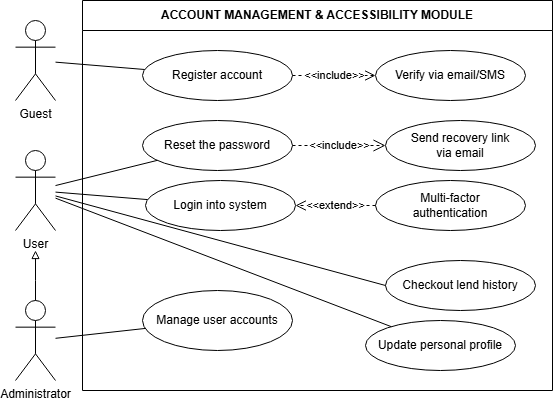
\includegraphics[width=0.8\linewidth]{Images/Quan_ly_tai_khoan_truy_cap.png}
    \vspace{10pt}
    \caption{Sơ đồ Use-case Quản lý Tài khoản và Truy cập Người dùng}
    \label{fig:usecase_account}
\end{figure}

\subsubsection{Đặc tả Chi tiết}

% --- UC: REGISTER ACCOUNT ---
\begin{longtable}{|p{3.5cm}|p{11.5cm}|}
    \hline
    \textbf{Tên Use-case} & \textbf{Đăng ký Tài khoản} \\
    \hline
    \textbf{Mã Use-case} & UC-ACC-01 \\
    \hline
    \textbf{Tổng quan} & Allows unregistered users to sign up and become system members. \\
    \hline
    \textbf{Tác nhân} & Khách \\
    \hline
    \textbf{Điều kiện tiên quyết} & Guest accesses the registration page of the system. \\
    \hline
    \textbf{Điều kiện kích hoạt} & Guest clicks the "Register" button. \\
    \hline
    \textbf{Luồng sự kiện} & 
    1. System displays the registration form.\newline
    2. Guest inputs required fields (Full name, Email, Password, etc.).\newline
    3. System validates input data integrity.\newline
    4. \textbf{[Bao gồm]} System executes "Send Verification Email/SMS" containing an OTP or activation link to the registered contact info.\newline
    5. Guest inputs the verification code or clicks the activation link.\newline
    6. System verifies the token, creates a new account, and persists it to the database.\newline
    7. System displays a success message. \\
    \hline
    \textbf{Điều kiện sau} & Account is created successfully and status transitions to "Activated". \\
    \hline
    \textbf{Ngoại lệ} & 
    Ex1: Email/Phone number already exists $\rightarrow$ System reports an error and requests re-entry.\newline
    Ex2: Invalid verification code entered beyond maximum attempts $\rightarrow$ Cancel registration session. \\
    \hline
    \caption{Đặc tả Use-case: Đăng ký Tài khoản}
\end{longtable}

\newpage
% --- UC: RESET PASSWORD ---
\begin{longtable}{|p{3.5cm}|p{11.5cm}|}
    \hline
    \textbf{Tên Use-case} & \textbf{Đặt lại Mật khẩu} \\
    \hline
    \textbf{Mã Use-case} & UC-ACC-02 \\
    \hline
    \textbf{Tổng quan} & Assists users in recovering account access when forgetting login passwords. \\
    \hline
    \textbf{Tác nhân} & Người dùng (Tất cả vai trò) \\
    \hline
    \textbf{Điều kiện tiên quyết} & User possesses an existing system account but cannot recall password. \\
    \hline
    \textbf{Điều kiện kích hoạt} & User clicks "Forgot Password" on the login view. \\
    \hline
    \textbf{Luồng sự kiện} & 
    1. System prompts user for registered email.\newline
    2. User inputs email and submits.\newline
    3. System verifies email existence in the database.\newline
    4. \textbf{[Bao gồm]} System triggers "Send Recovery Link via Email" flow.\newline
    5. User accesses the reset link received in email.\newline
    6. System renders password reset screen.\newline
    7. User inputs new password and confirms.\newline
    8. System hashes and updates new password, showing success alert. \\
    \hline
    \textbf{Điều kiện sau} & User password is updated successfully. \\
    \hline
    \textbf{Ngoại lệ} & 
    Ex1: Email does not exist $\rightarrow$ Display "No account found associated with this email".\newline
    Ex2: Reset link expired $\rightarrow$ Prompt user to restart the reset process. \\
    \hline
    \caption{Đặc tả Use-case: Đặt lại Mật khẩu}
\end{longtable}

% --- UC: USER LOGIN ---
\begin{longtable}{|p{3.5cm}|p{11.5cm}|}
    \hline
    \textbf{Tên Use-case} & \textbf{Đăng nhập Hệ thống} \\
    \hline
    \textbf{Mã Use-case} & UC-ACC-03 \\
    \hline
    \textbf{Tổng quan} & Authenticates user identity to grant system access matching role privileges. \\
    \hline
    \textbf{Tác nhân} & Người dùng (Tất cả vai trò) \\
    \hline
    \textbf{Điều kiện tiên quyết} & User possesses an active account in the system. \\
    \hline
    \textbf{Điều kiện kích hoạt} & User accesses the login view and enters credentials. \\
    \hline
    \textbf{Luồng sự kiện} & 
    1. User submits identity credentials (Email/Username) and Password.\newline
    2. System validates input formats and matches credentials against DB.\newline
    3. \textbf{[Mở rộng]} If Multi-Factor Authentication (MFA) is configured, system triggers "MFA Verification", requesting OTP from app/SMS.\newline
    4. Initializes user session (Session/JWT Token).\newline
    5. Redirects user to the dashboard corresponding to their assigned Role. \\
    \hline
    \textbf{Điều kiện sau} & User logs in successfully; system records login timestamp audit. \\
    \hline
    \textbf{Ngoại lệ} & 
    Ex1: Incorrect credentials $\rightarrow$ Display "Incorrect account or password".\newline
    Ex2: Account suspended $\rightarrow$ Display "Your account is locked. Please contact Admin".\newline
    Ex3: MFA code failed > 3 attempts $\rightarrow$ Lock login session temporarily for 15 minutes. \\
    \hline
    \caption{Đặc tả Use-case: Đăng nhập Hệ thống}
\end{longtable}

\newpage
% --- UC: UPDATE PROFILE ---
\begin{longtable}{|p{3.5cm}|p{11.5cm}|}
    \hline
    \textbf{Tên Use-case} & \textbf{Cập nhật Hồ sơ Người dùng} \\
    \hline
    \textbf{Mã Use-case} & UC-ACC-04 \\
    \hline
    \textbf{Tổng quan} & Allows users to modify personal profile information on the platform. \\
    \hline
    \textbf{Tác nhân} & Người dùng \\
    \hline
    \textbf{Điều kiện tiên quyết} & User is currently logged into the system. \\
    \hline
    \textbf{Điều kiện kích hoạt} & User accesses "Profile Settings" and selects "Edit". \\
    \hline
    \textbf{Luồng sự kiện} & 
    1. System populates form with current profile data.\newline
    2. User updates permissible fields (Phone, address, avatar image...).\newline
    3. User clicks "Save".\newline
    4. System validates field constraints.\newline
    5. Updates database record and displays success notification. \\
    \hline
    \textbf{Điều kiện sau} & User profile is updated. \\
    \hline
    \textbf{Ngoại lệ} & 
    Ex1: Invalid avatar format or file size exceeded $\rightarrow$ Warning alert and file rejection. \\
    \hline
    \caption{Đặc tả Use-case: Cập nhật Hồ sơ Người dùng}
\end{longtable}

% --- UC: VIEW BORROWING HISTORY ---
\begin{longtable}{|p{3.5cm}|p{11.5cm}|}
    \hline
    \textbf{Tên Use-case} & \textbf{Xem Lịch sử Mượn/Trả} \\
    \hline
    \textbf{Mã Use-case} & UC-ACC-05 \\
    \hline
    \textbf{Tổng quan} & Enables users to review past and active item borrowings along with their statuses. \\
    \hline
    \textbf{Tác nhân} & Người dùng \\
    \hline
    \textbf{Điều kiện tiên quyết} & User is logged into the system. \\
    \hline
    \textbf{Điều kiện kích hoạt} & User selects "Borrowing History" in personal dashboard. \\
    \hline
    \textbf{Luồng sự kiện} & 
    1. System receives user request.\newline
    2. Queries database for circulation records tied to user ID.\newline
    3. Renders loan list (Item title, borrow date, due date, return date, status, fines).\newline
    4. User can filter results by date range or status. \\
    \hline
    \textbf{Điều kiện sau} & System state remains unchanged. \\
    \hline
    \textbf{Ngoại lệ} & 
    Ex1: No loan records found $\rightarrow$ Display "You have no borrowing history". \\
    \hline
    \caption{Đặc tả Use-case: Xem Lịch sử Mượn/Trả}
\end{longtable}

\newpage
% --- UC: USER ACCOUNT MANAGEMENT (ADMIN) ---
\begin{longtable}{|p{3.5cm}|p{11.5cm}|}
    \hline
    \textbf{Tên Use-case} & \textbf{Quản lý Tài khoản Người dùng} \\
    \hline
    \textbf{Mã Use-case} & UC-ACC-06 \\
    \hline
    \textbf{Tổng quan} & Empowers administrators to search, view, authorize, activate, or suspend user accounts. \\
    \hline
    \textbf{Tác nhân} & Quản trị viên (Admin) \\
    \hline
    \textbf{Điều kiện tiên quyết} & Administrator is logged in with administrative access privileges. \\
    \hline
    \textbf{Điều kiện kích hoạt} & Admin navigates to "User Management" menu. \\
    \hline
    \textbf{Luồng sự kiện} & 
    1. System displays table of all user accounts.\newline
    2. Admin filters or searches accounts by role or account status.\newline
    3. Admin selects a specific user to perform actions (Lock/Unlock, Reset Password, Change Role).\newline
    4. Admin confirms the administrative operation.\newline
    5. System persists changes to DB and writes audit log.\newline
    6. System displays success confirmation. \\
    \hline
    \textbf{Điều kiện sau} & Target account status or permission set is updated. \\
    \hline
    \textbf{Ngoại lệ} & 
    Ex1: Admin attempts to lock their own account $\rightarrow$ System rejects action and raises logic violation error. \\
    \hline
    \caption{Đặc tả Use-case: Quản lý Tài khoản Người dùng}
\end{longtable}

% ======================================================================================
% 4.2 CATALOG AND AI METADATA MANAGEMENT
% ======================================================================================
\subsection{Quản lý Danh mục và Dữ liệu tả}

\subsubsection{Tổng quan}
\begin{figure}[H]
    \centering
    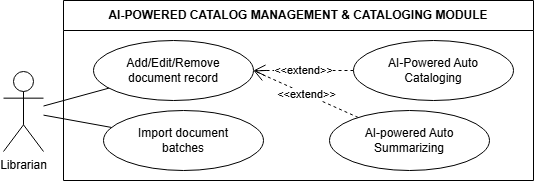
\includegraphics[width=0.8\linewidth]{Images/Quan_ly_danh_muc_bien_muc_AI.png}
    \vspace{10pt}
    \caption{Sơ đồ Use-case Quản lý Danh mục \& Dữ liệu tả AI}
    \label{fig:usecase_catalog}
\end{figure}

\subsubsection{Đặc tả Chi tiết}

% --- UC: ADD / EDIT / DELETE CATALOG RECORD ---
\begin{longtable}{|p{3.5cm}|p{11.5cm}|}
    \hline
    \textbf{Tên Use-case} & \textbf{Thêm / Sửa / Xóa Bản ghi Danh mục} \\
    \hline
    \textbf{Mã Use-case} & UC-CAT-01 \\
    \hline
    \textbf{Tổng quan} & Librarians perform catalog management operations (CRUD), updating metadata or removing lost/damaged copies. \\
    \hline
    \textbf{Tác nhân} & Thủ thư \\
    \hline
    \textbf{Điều kiện tiên quyết} & Librarian is logged into the system. \\
    \hline
    \textbf{Điều kiện kích hoạt} & Librarian navigates to "Catalog Management". \\
    \hline
    \textbf{Luồng sự kiện} & 
    1. System displays list of current catalog items.\newline
    2. Librarian selects action: Add New, Edit, or Delete.\newline
    3. If Delete: Librarian confirms deletion, system checks active loan constraints and executes Soft Delete.\newline
    4. If Add/Edit: System renders item form (Title, Author, ISBN, Category, Copies...).\newline
    \textit{** Extension Points:**}\newline
    - \textbf{[Mở rộng]} Librarian can execute \textit{"Biên mục Tự động qua ISBN"} (UC-CAT-03) to auto-fill form.\newline
    - \textbf{[Mở rộng]} Librarian can execute \textit{"Tóm tắt Tài liệu Tự động"} (UC-CAT-04) if description is missing.\newline
    5. Librarian reviews form fields and clicks "Save".\newline
    6. System validates fields, persists to DB, and displays success alert. \\
    \hline
    \textbf{Điều kiện sau} & Catalog record is updated successfully. \\
    \hline
    \textbf{Ngoại lệ} & 
    Ex1: Required fields missing $\rightarrow$ System highlights missing inputs and requests completion.\newline
    Ex2: Duplicate ISBN code $\rightarrow$ Display "ISBN already exists in catalog". \\
    \hline
    \caption{Đặc tả Use-case: Thêm / Sửa / Xóa Bản ghi Danh mục}
\end{longtable}

\newpage
% --- UC: BATCH CATALOG INGESTION ---
\begin{longtable}{|p{3.5cm}|p{11.5cm}|}
    \hline
    \textbf{Tên Use-case} & \textbf{Nhập Dữ liệu Danh mục Hàng loạt} \\
    \hline
    \textbf{Mã Use-case} & UC-CAT-02 \\
    \hline
    \textbf{Tổng quan} & Allows librarians to import large volumes of catalog records via standard data files (CSV, Excel). \\
    \hline
    \textbf{Tác nhân} & Thủ thư \\
    \hline
    \textbf{Điều kiện tiên quyết} & Librarian is logged into the system. \\
    \hline
    \textbf{Điều kiện kích hoạt} & Librarian clicks "Batch Import" in catalog management. \\
    \hline
    \textbf{Luồng sự kiện} & 
    1. System presents upload interface and sample template file.\newline
    2. Librarian uploads catalog dataset file.\newline
    3. System parses file and displays preview table distinguishing valid vs invalid records.\newline
    4. Librarian confirms import operation.\newline
    5. System writes valid rows to DB and generates execution report (success vs error row counts). \\
    \hline
    \textbf{Điều kiện sau} & Multiple catalog records added to system. \\
    \hline
    \textbf{Ngoại lệ} & 
    Ex1: Unsupported file format $\rightarrow$ System rejects upload: "Unsupported file format".\newline
    Ex2: File contains duplicate ISBNs $\rightarrow$ System skips duplicate lines, logs errors, and imports remaining valid records. \\
    \hline
    \caption{Đặc tả Use-case: Nhập Dữ liệu Danh mục Hàng loạt}
\end{longtable}

% --- UC: AUTOMATED CATALOGING VIA ISBN (AI) ---
\begin{longtable}{|p{3.5cm}|p{11.5cm}|}
    \hline
    \textbf{Tên Use-case} & \textbf{Biên mục Tự động qua ISBN} \\
    \hline
    \textbf{Mã Use-case} & UC-CAT-03 \\
    \hline
    \textbf{Tổng quan} & AI-assisted feature to automatically retrieve and populate book metadata (Title, Author, Publisher, Genre) from external APIs using ISBN lookup. \\
    \hline
    \textbf{Tác nhân} & Thủ thư \\
    \hline
    \textbf{Điều kiện tiên quyết} & Currently executing flow of "Thêm / Sửa / Xóa Bản ghi Danh mục". \\
    \hline
    \textbf{Điều kiện kích hoạt} & Librarian enters ISBN and clicks "Auto-Fetch Metadata". \\
    \hline
    \textbf{Luồng sự kiện} & 
    1. Librarian enters ISBN into corresponding input field.\newline
    2. System dispatches API request to open catalog endpoints (Google Books, Open Library).\newline
    3. System receives JSON response, parsing entity attributes.\newline
    4. System auto-populates form fields with parsed attributes.\newline
    5. Librarian reviews, edits if needed, and proceeds with base cataloging flow. \\
    \hline
    \textbf{Điều kiện sau} & Catalog form is auto-filled, reducing manual entry time for librarians. \\
    \hline
    \textbf{Ngoại lệ} & 
    Ex1: ISBN not found in external databases $\rightarrow$ System alerts "No metadata found, please enter manually".\newline
    Ex2: Third-party API timeout $\rightarrow$ System alerts timeout error and asks librarian to retry. \\
    \hline
    \caption{Đặc tả Use-case: Biên mục Tự động qua ISBN}
\end{longtable}

\newpage
% --- UC: AUTOMATED DOCUMENT SUMMARIZATION (AI) ---
\begin{longtable}{|p{3.5cm}|p{11.5cm}|}
    \hline
    \textbf{Tên Use-case} & \textbf{Tóm tắt Tài liệu Tự động} \\
    \hline
    \textbf{Mã Use-case} & UC-CAT-04 \\
    \hline
    \textbf{Tổng quan} & Uses Large Language Models (LLMs) to automatically generate concise abstract summaries (150-300 words) for catalog items lacking publisher descriptions. \\
    \hline
    \textbf{Tác nhân} & Thủ thư \\
    \hline
    \textbf{Điều kiện tiên quyết} & Executing "Thêm / Sửa / Xóa Bản ghi Danh mục" flow. Title and Author fields populated. \\
    \hline
    \textbf{Điều kiện kích hoạt} & Librarian clicks "Generate AI Summary" in Description field. \\
    \hline
    \textbf{Luồng sự kiện} & 
    1. System collects existing item fields (Title, Author, Category).\newline
    2. System formats prompt payload and sends to AI Engine (e.g., Gemini API).\newline
    3. AI Engine processes payload and returns summary text.\newline
    4. System populates text into Description field, automatically tagging "(AI-generated summary)".\newline
    5. Librarian reviews, edits, or requests regeneration. \\
    \hline
    \textbf{Điều kiện sau} & Item receives concise abstract summary, aiding reader discovery. \\
    \hline
    \textbf{Ngoại lệ} & 
    Ex1: Insufficient metadata input causing inaccurate AI synthesis $\rightarrow$ Generic output returned; librarian discards and clears output. \\
    \hline
    \caption{Đặc tả Use-case: Tóm tắt Tài liệu Tự động}
\end{longtable}

% ======================================================================================
% 4.3 CIRCULATION MANAGEMENT
% ======================================================================================
\subsection{Quản lý Lưu thông Tài liệu}

\subsubsection{Tổng quan}
\begin{figure}[H]
    \centering
    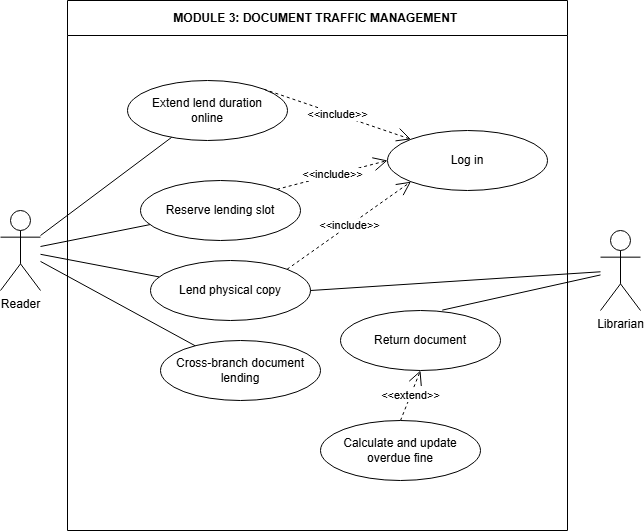
\includegraphics[width=0.8\linewidth]{Images/Quan_ly_luu_thong.png}
    \vspace{10pt}
    \caption{Sơ đồ Use-case Quản lý Lưu thông Tài liệu}
    \label{fig:usecase_circulation}
\end{figure}

\subsubsection{Đặc tả Chi tiết}

% --- UC: BORROW PHYSICAL MATERIAL ---
\begin{longtable}{|p{3.5cm}|p{11.5cm}|}
    \hline
    \textbf{Tên Use-case} & \textbf{Mượn Tài liệu Vật lý} \\
    \hline
    \textbf{Mã Use-case} & UC-CIR-01 \\
    \hline
    \textbf{Tổng quan} & Allows readers to borrow physical materials available at the library counter assisted by a librarian. \\
    \hline
    \textbf{Tác nhân} & Độc giả, Thủ thư \\
    \hline
    \textbf{Điều kiện tiên quyết} & Reader and Librarian possess valid active accounts. Reader has no card suspension or unpaid fines exceeding threshold. \\
    \hline
    \textbf{Điều kiện kích hoạt} & Reader presents items and membership card at circulation desk. \\
    \hline
    \textbf{Luồng sự kiện} & 
    1. \textbf{[Bao gồm]} Librarian logs into circulation module.\newline
    2. Librarian scans Reader membership barcode/ID.\newline
    3. System loads Reader profile, checking borrowing eligibility and fine status.\newline
    4. Librarian scans barcode on each checkout item.\newline
    5. System checks active loan limits against role allowance.\newline
    6. System creates loan record, calculating due dates based on item policy rules.\newline
    7. System updates copy status in inventory to "Checked Out" and decrements available count.\newline
    8. Librarian hands items to Reader; transaction completes. \\
    \hline
    \textbf{Điều kiện sau} & Loan record created in system; transaction logged. \\
    \hline
    \textbf{Ngoại lệ} & 
    Ex1: Reader reached maximum borrowing limit $\rightarrow$ Error alert "Loan limit exceeded"; reader must return existing items first.\newline
    Ex2: Item scanned is on hold for another patron $\rightarrow$ Warning alert; librarian retains item for hold queue. \\
    \hline
    \caption{Đặc tả Use-case: Mượn Tài liệu Vật lý}
\end{longtable}

\newpage
% --- UC: RETURN MATERIAL ---
\begin{longtable}{|p{3.5cm}|p{11.5cm}|}
    \hline
    \textbf{Tên Use-case} & \textbf{Trả Tài liệu} \\
    \hline
    \textbf{Mã Use-case} & UC-CIR-02 \\
    \hline
    \textbf{Tổng quan} & Processes returned physical materials, closes active loan records, and updates copy availability in inventory. \\
    \hline
    \textbf{Tác nhân} & Thủ thư \\
    \hline
    \textbf{Điều kiện tiên quyết} & Items are associated with active open loan records. \\
    \hline
    \textbf{Điều kiện kích hoạt} & Reader returns items at circulation desk. \\
    \hline
    \textbf{Luồng sự kiện} & 
    1. \textbf{[Bao gồm]} Librarian logs into circulation module.\newline
    2. Librarian scans item barcode.\newline
    3. System retrieves associated active loan record.\newline
    4. System compares return date against scheduled due date.\newline
    \textit{** Extension Points:**}\newline
    - \textbf{[Mở rộng]} If return date exceeds due date, system triggers "Tính và Thu Phạt Quá hạn" (UC-CIR-03).\newline
    5. Updates loan status to "Completed".\newline
    6. System verifies hold queue status for returned item:\newline
    - If hold exists: Set status to "Awaiting Pickup" and send notification to next patron.\newline
    - If no hold: Set status to "Available" and increment copy inventory count. \\
    \hline
    \textbf{Điều kiện sau} & Loan record closed. Item marked available for next transaction. \\
    \hline
    \textbf{Ngoại lệ} & 
    Ex1: Barcode damaged/unreadable $\rightarrow$ Librarian performs manual lookup by title and borrower ID. \\
    \hline
    \caption{Đặc tả Use-case: Trả Tài liệu}
\end{longtable}

% --- UC: CALCULATE OVERDUE FINES ---
\begin{longtable}{|p{3.5cm}|p{11.5cm}|}
    \hline
    \textbf{Tên Use-case} & \textbf{Tính và Thu Phạt Quá hạn} \\
    \hline
    \textbf{Mã Use-case} & UC-CIR-03 \\
    \hline
    \textbf{Tổng quan} & Automatically computes fine amounts when items are returned past due dates. \\
    \hline
    \textbf{Tác nhân} & Thủ thư \\
    \hline
    \textbf{Điều kiện tiên quyết} & Triggered from "Trả Tài liệu" when system detects overdue return. \\
    \hline
    \textbf{Điều kiện kích hoạt} & Return Date > Due Date in loan record. \\
    \hline
    \textbf{Luồng sự kiện} & 
    1. System computes overdue days: (Actual Return Date - Due Date).\newline
    2. Fetches daily fine rate applicable to material type (configured by Admin).\newline
    3. Calculates total fine amount (Overdue Days $\times$ Daily Rate).\newline
    4. Displays fine calculation on librarian view.\newline
    5. Librarian notifies reader. If reader pays immediately, receipt is generated; otherwise fine is posted to reader ledger. \\
    \hline
    \textbf{Điều kiện sau} & Fine record updated on reader profile or marked as paid. \\
    \hline
    \textbf{Ngoại lệ} & 
    Ex1: Official holidays fall within overdue range $\rightarrow$ System automatically excludes official library holidays from overdue day count. \\
    \hline
    \caption{Đặc tả Use-case: Tính và Thu Phạt Quá hạn}
\end{longtable}

\newpage
% --- UC: ONLINE LOAN RENEWAL ---
\begin{longtable}{|p{3.5cm}|p{11.5cm}|}
    \hline
    \textbf{Tên Use-case} & \textbf{Gia hạn Mượn Trực tuyến} \\
    \hline
    \textbf{Mã Use-case} & UC-CIR-04 \\
    \hline
    \textbf{Tổng quan} & Allows readers to extend loan periods online without physically visiting the library. \\
    \hline
    \textbf{Tác nhân} & Độc giả \\
    \hline
    \textbf{Điều kiện tiên quyết} & Item is not overdue and renewal limit has not been reached. \\
    \hline
    \textbf{Điều kiện kích hoạt} & Reader clicks "Renew" in active loans dashboard. \\
    \hline
    \textbf{Luồng sự kiện} & 
    1. \textbf{[Bao gồm]} Reader logs into system portal.\newline
    2. System verifies renewal eligibility:\newline
    - Has maximum renewal limit been reached for item?\newline
    - Does an active hold request exist from another user?\newline
    3. If eligible, system extends due date by configured extension period.\newline
    4. System updates loan record and increments renewal counter.\newline
    5. Displays "Renewal Successful" along with new due date. \\
    \hline
    \textbf{Điều kiện sau} & Item due date is extended. \\
    \hline
    \textbf{Ngoại lệ} & 
    Ex1: Item has active hold request $\rightarrow$ System rejects renewal: "Item requested by another user, please return on time". \\
    \hline
    \caption{Đặc tả Use-case: Gia hạn Mượn Trực tuyến}
\end{longtable}

% --- UC: PLACE ITEM HOLD ---
\begin{longtable}{|p{3.5cm}|p{11.5cm}|}
    \hline
    \textbf{Tên Use-case} & \textbf{Đặt Giữ chỗ Tài liệu} \\
    \hline
    \textbf{Mã Use-case} & UC-CIR-05 \\
    \hline
    \textbf{Tổng quan} & Enables readers to join a reservation queue for items currently out of stock. \\
    \hline
    \textbf{Tác nhân} & Độc giả \\
    \hline
    \textbf{Điều kiện tiên quyết} & Target item status is "All Copies Checked Out". \\
    \hline
    \textbf{Điều kiện kích hoạt} & Reader clicks "Place Hold" on item detail view. \\
    \hline
    \textbf{Luồng sự kiện} & 
    1. \textbf{[Bao gồm]} Reader logs into system portal.\newline
    2. System verifies Reader does not currently hold an active loan for same title.\newline
    3. System appends Reader ID to item reservation queue.\newline
    4. Interface displays "Hold Placed Successfully" showing queue position.\newline
    5. Upon item return, system holds copy and alerts queue position \#1 patron. \\
    \hline
    \textbf{Điều kiện sau} & Reservation saved; renewal blocked for current borrower. \\
    \hline
    \textbf{Ngoại lệ} & 
    Ex1: Reader has unpaid fines or card suspension $\rightarrow$ System rejects hold request. \\
    \hline
    \caption{Đặc tả Use-case: Place Item Hold}
\end{longtable}

\newpage
% --- UC: INTER-BRANCH LOAN REQUEST ---
\begin{longtable}{|p{3.5cm}|p{11.5cm}|}
    \hline
    \textbf{Tên Use-case} & \textbf{Yêu cầu Mượn Liên Chi nhánh} \\
    \hline
    \textbf{Mã Use-case} & UC-CIR-06 \\
    \hline
    \textbf{Tổng quan} & Allows readers to request item transfers from another branch library to their local campus library for pickup. \\
    \hline
    \textbf{Tác nhân} & Độc giả \\
    \hline
    \textbf{Điều kiện tiên quyết} & Multi-branch network enabled. Item unavailable locally but available at another branch. \\
    \hline
    \textbf{Điều kiện kích hoạt} & Reader clicks "Request Inter-Branch Transfer" on book detail page. \\
    \hline
    \textbf{Luồng sự kiện} & 
    1. \textbf{[Bao gồm]} Reader logs into system portal.\newline
    2. System prompts Reader to select preferred pickup branch.\newline
    3. Reader confirms request.\newline
    4. System creates inter-branch transfer ticket sent to holding branch.\newline
    5. Holding librarian packages item; status changes to "In Transit".\newline
    6. Upon arrival at destination branch, automated notification alerts Reader for pickup. \\
    \hline
    \textbf{Điều kiện sau} & Physical transfer logged and inventory updated across branches. \\
    \hline
    \textbf{Ngoại lệ} & 
    Ex1: Last available copy borrowed before request processing $\rightarrow$ Cancel request and suggest standard hold queue. \\
    \hline
    \caption{Đặc tả Use-case: Yêu cầu Mượn Liên Chi nhánh}
\end{longtable}

% ======================================================================================
% 4.4 RESOURCE ACCESS AND EXPLOITATION
% ======================================================================================
\subsection{Truy cập và Khai thác Tài nguyên}

\subsubsection{Tổng quan}
\begin{figure}[H]
    \centering
    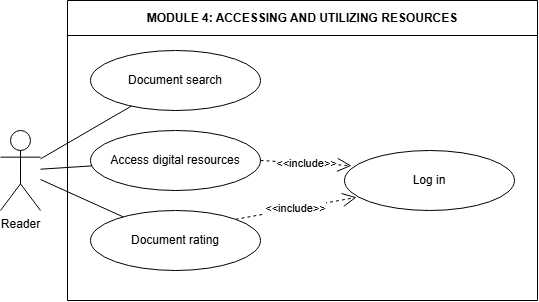
\includegraphics[width=0.8\linewidth]{Images/Truy_cap_khai_thac_tai_nguyen.png}
    \vspace{10pt}
    \caption{Sơ đồ Use-case Truy cập \& Khai thác Tài nguyên}
    \label{fig:usecase_exploration}
\end{figure}

\subsubsection{Đặc tả Chi tiết}

% --- UC: DOCUMENT SEARCH ---
\begin{longtable}{|p{3.5cm}|p{11.5cm}|}
    \hline
    \textbf{Tên Use-case} & \textbf{Tìm kiếm Danh mục Tài liệu} \\
    \hline
    \textbf{Mã Use-case} & UC-EXP-01 \\
    \hline
    \textbf{Tổng quan} & Allows readers to search library catalog records via keywords (Title, Author, Genre, ISBN). \\
    \hline
    \textbf{Tác nhân} & Độc giả (Bao gồm cả khách chưa xác thực) \\
    \hline
    \textbf{Điều kiện tiên quyết} & System online with active DB connection. \\
    \hline
    \textbf{Điều kiện kích hoạt} & Reader inputs query string and submits search. \\
    \hline
    \textbf{Luồng sự kiện} & 
    1. Reader selects search filter scope (All, Title, Author...) and enters query.\newline
    2. System queries catalog database indexes.\newline
    3. System returns paginated match results.\newline
    4. Renders item cards (Cover image, Title, Author, Year, Availability Status).\newline
    5. Reader clicks item card to open detail view. \\
    \hline
    \textbf{Điều kiện sau} & System state remains unchanged. \\
    \hline
    \textbf{Ngoại lệ} & 
    Ex1: No items match query $\rightarrow$ Display "No results found" with spelling/keyword suggestions. \\
    \hline
    \caption{Đặc tả Use-case: Tìm kiếm Danh mục Tài liệu}
\end{longtable}

% \newpage
% % --- UC: ACCESS DIGITAL RESOURCES (chưa triển khai) ---
% \begin{longtable}{|p{3.5cm}|p{11.5cm}|}
%     \hline
%     \textbf{Tên Use-case} & \textbf{Access Digital Resources} \\\
%     \hline
%     \textbf{Mã Use-case} & UC-EXP-02 \\\
%     \hline
%     \textbf{Tổng quan} & Enables readers to stream/read digital materials (E-books, PDFs) online. \\\
%     \hline
%     \textbf{Tác nhân} & Độc giả \\\
%     \hline
%     \textbf{Điều kiện tiên quyết} & Item possesses digital file format. \\\
%     \hline
%     \textbf{Điều kiện kích hoạt} & Reader clicks ``Read Online'' on item page. \\\
%     \hline
%     \textbf{Luồng sự kiện} &
%     1. \textbf{[Bao gồm]} System checks authentication, prompting login if needed.\newline
%     2. System verifies Reader digital access privileges.\newline
%     3. System checks concurrent license access limits (e.g., max 5 concurrent readers).\newline
%     4. If approved, opens embedded web PDF/ePUB viewer.\newline
%     5. Logs digital reading session. \\\
%     \hline
%     \textbf{Điều kiện sau} & Digital reading session established. \\\
%     \hline
%     \textbf{Ngoại lệ} &
%     Ex1: Concurrent user limit reached $\rightarrow$ Display ``All digital licenses currently in use. Please try again later''. \\\
%     \hline
%     \caption{Đặc tả Use-case: Access Digital Resources (not implemented)}
% \end{longtable}

% --- UC: RATE AND REVIEW MATERIALS ---
\begin{longtable}{|p{3.5cm}|p{11.5cm}|}
    \hline
    \textbf{Tên Use-case} & \textbf{Đánh giá và Nhận xét Tài liệu} \\
    \hline
    \textbf{Mã Use-case} & UC-EXP-03 \\
    \hline
    \textbf{Tổng quan} & Allows readers to leave 1-5 star ratings and written reviews for items they have read. \\
    \hline
    \textbf{Tác nhân} & Độc giả \\
    \hline
    \textbf{Điều kiện tiên quyết} & Reader has borrowed the physical item (preventing spam). \\
    \hline
    \textbf{Điều kiện kích hoạt} & Reader clicks "Write a Review" on book page. \\
    \hline
    \textbf{Luồng sự kiện} & 
    1. \textbf{[Bao gồm]} System verifies login status.\newline
    2. System verifies loan history against target item.\newline
    3. Renders rating selector (1-5 stars) and review text area.\newline
    4. Reader submits rating and optional review.\newline
    5. System checks content moderation filters.\newline
    6. Saves rating, updates item average rating score.\newline
    7. Displays success alert and refreshes view. \\
    \hline
    \textbf{Điều kiện sau} & Review saved; average item score updated. \\
    \hline
    \textbf{Ngoại lệ} & 
    Ex1: Reader has not borrowed item $\rightarrow$ Hide review button or display "You must borrow this item before submitting a review".\newline
    Ex2: Review contains profanity $\rightarrow$ Block submission with moderation warning. \\
    \hline
    \caption{Đặc tả Use-case: Đánh giá và Nhận xét Tài liệu}
\end{longtable}

% ======================================================================================
% 4.5 INTELLIGENT INTERACTION AND AI
% ======================================================================================
\subsection{Tương tác Thông minh}

\subsubsection{Tổng quan}
\begin{figure}[H]
    \centering
    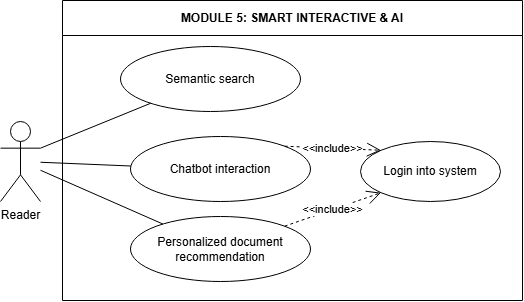
\includegraphics[width=0.8\linewidth]{Images/Tuong_tac_thong_minh_AI.png}
    \vspace{10pt}
    \caption{Sơ đồ Use-case Tương tác Thông minh \& AI}
    \label{fig:usecase_smart_ai}
\end{figure}

\subsubsection{Đặc tả Chi tiết}

% --- UC: NATURAL LANGUAGE SEARCH ---
\begin{longtable}{|p{3.5cm}|p{11.5cm}|}
    \hline
    \textbf{Tên Use-case} & \textbf{Tìm kiếm Ngôn ngữ Tự nhiên} \\
    \hline
    \textbf{Mã Use-case} & UC-AI-01 \\
    \hline
    \textbf{Tổng quan} & Allows readers to search catalog items using conversational phrases (e.g., "introductory artificial intelligence textbooks") rather than exact keywords. \\
    \hline
    \textbf{Tác nhân} & Độc giả \\
    \hline
    \textbf{Điều kiện tiên quyết} & System AI NLP module operational. \\
    \hline
    \textbf{Điều kiện kích hoạt} & Reader inputs phrase into Smart Search bar and submits. \\
    \hline
    \textbf{Luồng sự kiện} & 
    1. Reader enters natural language query.\newline
    2. NLP module processes query via Intent Analysis \& Entity Extraction (genre, topic, target level).\newline
    3. System converts entities into vector embeddings or metadata filter trees.\newline
    4. Executes vector similarity search (pgvector) and semantic ranking.\newline
    5. Renders ranked search results sorted by semantic relevance scores. \\
    \hline
    \textbf{Điều kiện sau} & Semantic search results rendered with related topic tags. \\
    \hline
    \textbf{Ngoại lệ} & 
    Ex1: Irrelevant or meaningless phrase $\rightarrow$ AI assistant prompts "No matching documents found. Try phrases like...".\newline
    Ex2: AI service offline $\rightarrow$ System falls back to full-text keyword search and alerts "Smart search temporarily under maintenance". \\
    \hline
    \caption{Đặc tả Use-case: Tìm kiếm Ngôn ngữ Tự nhiên}
\end{longtable}

\newpage
% --- UC: CHATBOT VIRTUAL ASSISTANT ---
\begin{longtable}{|p{3.5cm}|p{11.5cm}|}
    \hline
    \textbf{Tên Use-case} & \textbf{Tương tác với Chatbot Trợ lý ảo} \\
    \hline
    \textbf{Mã Use-case} & UC-AI-02 \\
    \hline
    \textbf{Tổng quan} & Readers interact with an AI Chatbot for policy inquiries, opening hours, or checking personal account loan status. \\
    \hline
    \textbf{Tác nhân} & Độc giả \\
    \hline
    \textbf{Điều kiện tiên quyết} & AI Chatbot service online. \\
    \hline
    \textbf{Điều kiện kích hoạt} & Reader opens Chatbot widget window. \\
    \hline
    \textbf{Luồng sự kiện} & 
    1. \textbf{[Bao gồm]} System prompts login if unauthenticated for personalized responses.\newline
    2. Chatbot interface displays welcome message and quick action buttons (FAQ, My Loans, Book Suggestions).\newline
    3. Reader types message or selects quick prompt.\newline
    4. Chatbot (LLM) analyzes context:\newline
    - General FAQ: Retrieves answer from RAG knowledge base.\newline
    - Account query (e.g., "What books do I owe?"): Chatbot queries backend API using Reader ID and synthesizes response.\newline
    5. Renders conversational response in chat widget. \\
    \hline
    \textbf{Điều kiện sau} & Chat transcript saved for audit logging and AI refinement. \\
    \hline
    \textbf{Ngoại lệ} & 
    Ex1: Query out of scope $\rightarrow$ Response: "I am a library assistant. Please contact staff at hotline for special inquiries." \\
    \hline
    \caption{Đặc tả Use-case: Tương tác với Chatbot Trợ lý ảo}
\end{longtable}

\newpage
% --- UC: PERSONALIZED RECOMMENDATIONS ---
% \begin{longtable}{|p{3.5cm}|p{11.5cm}|}
%     \hline
%     \textbf{Tên Use-case} & \textbf{Xem Gợi ý Cá nhân hóa} \\
%     \hline
%     \textbf{Mã Use-case} & UC-AI-03 \\
%     \hline
%     \textbf{Tổng quan} & Provides readers with tailored book recommendations generated from loan history, search logs, and collaborative user behavior. \\
%     \hline
%     \textbf{Tác nhân} & Độc giả \\
%     \hline
%     \textbf{Điều kiện tiên quyết} & AI Recommendation engine online. \\
%     \hline
%     \textbf{Điều kiện kích hoạt} & Reader opens homepage dashboard or "Recommended For You" view. \\
%     \hline
%     \textbf{Luồng sự kiện} & 
%     1. \textbf{[Bao gồm]} Reader logs into system.\newline
%     2. System aggregates user signals: loan history, recent searches, ratings.\newline
%     3. System sends telemetry to Recommendation Engine.\newline
%     4. Engine executes Collaborative Filtering and Content-Based Filtering models.\newline
%     5. Filters out items currently checked out or held by user.\newline
%     6. Displays "Recommended For You" grid with brief rationale tags (e.g., "Because you read Title X..."). \\
%     \hline
%     \textbf{Điều kiện sau} & Interface presents personalized recommendations. \\
%     \hline
%     \textbf{Ngoại lệ} & 
%     Ex1: New account with no history (Cold Start) $\rightarrow$ Display "Trending Titles" or "New Arrivals" fallback. \\
%     \hline
%     \caption{Đặc tả Use-case: Xem Gợi ý Cá nhân hóa}
% \end{longtable}

% ======================================================================================
% 4.6 NOTIFICATIONS AND COMMUNICATION
% ======================================================================================
\subsection{Thông báo và Tương tác}

\subsubsection{Tổng quan}
\begin{figure}[H]
    \centering
    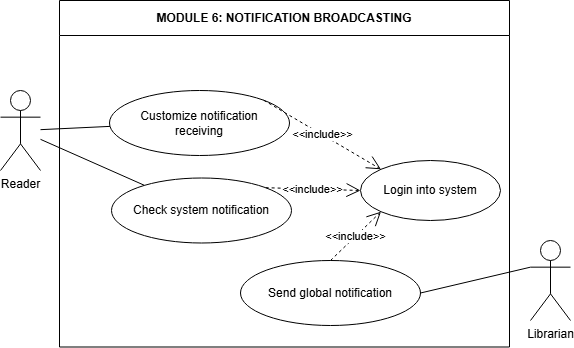
\includegraphics[width=0.8\linewidth]{Images/Thong_bao_truyen_thong.png}
    \vspace{10pt}
    \caption{Sơ đồ Use-case Thông báo \& Tương tác}
    \label{fig:usecase_notifications}
\end{figure}

\subsubsection{Đặc tả Chi tiết}

% --- UC: NOTIFICATION PREFERENCES ---
\begin{longtable}{|p{3.5cm}|p{11.5cm}|}
    \hline
    \textbf{Tên Use-case} & \textbf{Cấu hình Tùy chọn Thông báo} \\
    \hline
    \textbf{Mã Use-case} & UC-NOT-01 \\
    \hline
    \textbf{Tổng quan} & Allows readers to customize delivery channels (Email, SMS, In-app) and event alerts (Due Reminders, Hold Pickups, System News). \\
    \hline
    \textbf{Tác nhân} & Độc giả \\
    \hline
    \textbf{Điều kiện tiên quyết} & Reader possesses valid account. \\
    \hline
    \textbf{Điều kiện kích hoạt} & Reader opens "Notification Settings" in profile view. \\
    \hline
    \textbf{Luồng sự kiện} & 
    1. \textbf{[Bao gồm]} System prompts login verification.\newline
    2. System loads and renders current notification configuration toggles.\newline
    3. Reader toggles preferences for channels and event categories.\newline
    4. Reader clicks "Save Settings".\newline
    5. System validates and persists configuration to DB.\newline
    6. Displays "Notification preferences saved successfully". \\
    \hline
    \textbf{Điều kiện sau} & System dispatches notifications strictly per user preferences. \\
    \hline
    \textbf{Ngoại lệ} & 
    Ex1: SMS toggled on without phone number in profile $\rightarrow$ Warning alert requesting phone number update first. \\
    \hline
    \caption{Đặc tả Use-case: Cấu hình Tùy chọn Thông báo}
\end{longtable}

\newpage
% --- UC: VIEW SYSTEM NOTIFICATIONS ---
\begin{longtable}{|p{3.5cm}|p{11.5cm}|}
    \hline
    \textbf{Tên Use-case} & \textbf{Xem Thông báo Hệ thống} \\
    \hline
    \textbf{Mã Use-case} & UC-NOT-02 \\
    \hline
    \textbf{Tổng quan} & Enables users to review alerts and reminders directly within the web app interface. \\
    \hline
    \textbf{Tác nhân} & Độc giả \\
    \hline
    \textbf{Điều kiện tiên quyết} & User has incoming notification records. \\
    \hline
    \textbf{Điều kiện kích hoạt} & User clicks "Bell" icon (Notification Center) on top navbar. \\
    \hline
    \textbf{Luồng sự kiện} & 
    1. \textbf{[Bao gồm]} System verifies user login.\newline
    2. Queries notification table by User ID sorted by timestamp desc.\newline
    3. Renders notification panel distinguishing read vs unread items.\newline
    4. User clicks notification item to view details.\newline
    5. System marks notification as "Read" and decrements unread badge count. \\
    \hline
    \textbf{Điều kiện sau} & Notification status updated to "Read". \\
    \hline
    \textbf{Ngoại lệ} & 
    Ex1: Notification panel empty $\rightarrow$ Display "You have no new notifications". \\
    \hline
    \caption{Đặc tả Use-case: Xem Thông báo Hệ thống}
\end{longtable}

% --- UC: BROADCAST MASS NOTIFICATIONS ---
\begin{longtable}{|p{3.5cm}|p{11.5cm}|}
    \hline
    \textbf{Tên Use-case} & \textbf{Phát Thông báo Đại chúng} \\
    \hline
    \textbf{Mã Use-case} & UC-NOT-03 \\
    \hline
    \textbf{Tổng quan} & Allows Librarians to create and send general announcements (holiday closures, maintenance, policy updates) to all or targeted reader groups. \\
    \hline
    \textbf{Tác nhân} & Thủ thư \\
    \hline
    \textbf{Điều kiện tiên quyết} & Librarian active with broadcast privileges. \\
    \hline
    \textbf{Điều kiện kích hoạt} & Librarian accesses "Communication Management" tool in admin portal. \\
    \hline
    \textbf{Luồng sự kiện} & 
    1. \textbf{[Bao gồm]} System verifies Librarian session and privileges.\newline
    2. Renders broadcast creation form.\newline
    3. Librarian inputs: Title, Content, Channel (In-app, Email), Target Group (All, Students, Faculty).\newline
    4. Librarian clicks "Send Broadcast".\newline
    5. System prompts confirmation dialog.\newline
    6. System enqueues notification payload in Message Queue for dispatch.\newline
    7. Displays success confirmation and logs administrative action. \\
    \hline
    \textbf{Điều kiện sau} & Broadcast logged and dispatched to target users. \\
    \hline
    \textbf{Ngoại lệ} & 
    Ex1: Empty title or body $\rightarrow$ Disable send button and alert "Please enter complete broadcast content". \\
    \hline
    \caption{Đặc tả Use-case: Phát Thông báo Đại chúng}
\end{longtable}

% ======================================================================================
% 4.7 REPORTING AND SYSTEM ADMINISTRATION
% ======================================================================================
\subsection{Báo cáo và Quản trị Hệ thống}

\subsubsection{Tổng quan}
\begin{figure}[H]
    \centering
    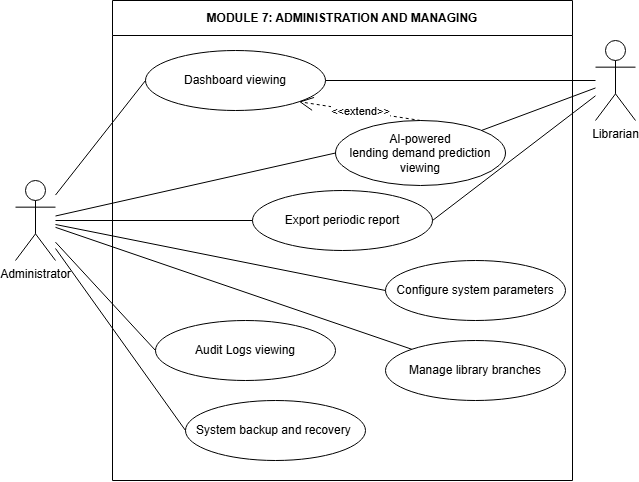
\includegraphics[width=0.8\linewidth]{Images/Bao_cao_quan_tri.png}
    \vspace{10pt}
    \caption{Sơ đồ Use-case Báo cáo \& Quản trị Hệ thống}
    \label{fig:usecase_admin}
\end{figure}

\subsubsection{Đặc tả Chi tiết}

% --- UC: VIEW DASHBOARD ---
\begin{longtable}{|p{3.5cm}|p{11.5cm}|}
    \hline
    \textbf{Tên Use-case} & \textbf{Xem Bảng điều khiển Vận hành} \\
    \hline
    \textbf{Mã Use-case} & UC-ADM-01 \\
    \hline
    \textbf{Tổng quan} & Provides real-time dashboard visualization of key operational metrics (active loans, overdue items, traffic). \\
    \hline
    \textbf{Tác nhân} & Quản trị viên (Admin), Thủ thư \\
    \hline
    \textbf{Điều kiện tiên quyết} & User logged in as Admin or Librarian. \\
    \hline
    \textbf{Điều kiện kích hoạt} & User opens administrative homepage. \\
    \hline
    \textbf{Luồng sự kiện} & 
    1. System receives request.\newline
    2. Queries DB aggregating real-time daily/weekly metrics.\newline
    3. Renders charts and metric summary cards. \\
    \hline
    \textbf{Điều kiện sau} & System data state remains unchanged. \\
    \hline
    \textbf{Ngoại lệ} & 
    Ex1: DB load high $\rightarrow$ Display cached dashboard data with refresh timestamp notice. \\
    \hline
    \caption{Đặc tả Use-case: Xem Bảng điều khiển Vận hành}
\end{longtable}

\newpage
% --- UC: EXPORT PERIODIC REPORTS ---
\begin{longtable}{|p{3.5cm}|p{11.5cm}|}
    \hline
    \textbf{Tên Use-case} & \textbf{Xuất Báo cáo Thống kê Định kỳ} \\
    \hline
    \textbf{Mã Use-case} & UC-ADM-02 \\
    \hline
    \textbf{Tổng quan} & Supports exporting library metrics and audit data to standard formats (PDF, CSV, Excel) for archiving and reporting. \\
    \hline
    \textbf{Tác nhân} & Quản trị viên (Admin), Thủ thư \\
    \hline
    \textbf{Điều kiện tiên quyết} & User logged in with report export privileges. \\
    \hline
    \textbf{Điều kiện kích hoạt} & User opens "Statistical Reports" and selects "Export Data". \\
    \hline
    \textbf{Luồng sự kiện} & 
    1. System renders export configuration modal.\newline
    2. User selects report type (Top Borrowed, Fine Income, Overdues), date range, and export format.\newline
    3. User clicks "Export".\newline
    4. System compiles dataset and generates file artifact.\newline
    5. File download triggers automatically on client browser. \\
    \hline
    \textbf{Điều kiện sau} & Report artifact generated and downloaded. \\
    \hline
    \textbf{Ngoại lệ} & 
    Ex1: No records match date range $\rightarrow$ Warning alert "No data available for selected period". \\
    \hline
    \caption{Đặc tả Use-case: Xuất Báo cáo Thống kê Định kỳ}
\end{longtable}

% --- UC: CONFIGURE SYSTEM PARAMETERS ---
\begin{longtable}{|p{3.5cm}|p{11.5cm}|}
    \hline
    \textbf{Tên Use-case} & \textbf{Cấu hình Tham số Hệ thống} \\
    \hline
    \textbf{Mã Use-case} & UC-ADM-04 \\
    \hline
    \textbf{Tổng quan} & Configures core operational library rules: loan limits, loan durations, and daily overdue fine rates per item type. \\
    \hline
    \textbf{Tác nhân} & Quản trị viên (Admin) \\
    \hline
    \textbf{Điều kiện tiên quyết} & Admin logged into system. \\
    \hline
    \textbf{Điều kiện kích hoạt} & Admin opens "System Settings". \\
    \hline
    \textbf{Luồng sự kiện} & 
    1. System displays current global system settings.\newline
    2. Admin modifies values (e.g., fine rate adjustment).\newline
    3. Admin clicks "Save Configuration".\newline
    4. System validates parameters.\newline
    5. Updates DB and records entry in Audit Log. \\
    \hline
    \textbf{Điều kiện sau} & System calculations immediately apply updated configuration settings. \\
    \hline
    \textbf{Ngoại lệ} & 
    Ex1: Invalid parameter input (negative values) $\rightarrow$ Reject save and display validation error. \\
    \hline
    \caption{Đặc tả Use-case: Cấu hình Tham số Hệ thống}
\end{longtable}

% --- UC: MANAGE BRANCHES ---
\begin{longtable}{|p{3.5cm}|p{11.5cm}|}
    \hline
    \textbf{Tên Use-case} & \textbf{Quản lý Chi nhánh Thư viện} \\
    \hline
    \textbf{Mã Use-case} & UC-ADM-05 \\
    \hline
    \textbf{Tổng quan} & Adds, edits, or deactivates affiliated branch libraries, managing physical network topology. \\
    \hline
    \textbf{Tác nhân} & Quản trị viên (Admin) \\
    \hline
    \textbf{Điều kiện tiên quyết} & Admin logged into system. \\
    \hline
    \textbf{Điều kiện kích hoạt} & Admin selects "Branch Management". \\
    \hline
    \textbf{Luồng sự kiện} & 
    1. System renders active branch list.\newline
    2. Admin selects Add New, Edit, or Remove.\newline
    3. Admin enters branch attributes (Name, Address, Contact, Manager).\newline
    4. Admin clicks "Save".\newline
    5. System updates records and displays success alert. \\
    \hline
    \textbf{Điều kiện sau} & Branch directory updated. \\
    \hline
    \textbf{Ngoại lệ} & 
    Ex1: Attempting to delete branch with active inventory or staff $\rightarrow$ System prevents deletion to maintain referential integrity. \\
    \hline
    \caption{Đặc tả Use-case: Quản lý Chi nhánh Thư viện}
\end{longtable}

\newpage
% --- UC: VIEW AUDIT LOGS ---
\begin{longtable}{|p{3.5cm}|p{11.5cm}|}
    \hline
    \textbf{Tên Use-case} & \textbf{Xem Nhật ký Kiểm toán} \\
    \hline
    \textbf{Mã Use-case} & UC-ADM-06 \\
    \hline
    \textbf{Tổng quan} & Inspects historical logs of critical administrative actions (who did what, when) for security auditing. \\
    \hline
    \textbf{Tác nhân} & Quản trị viên (Admin) \\
    \hline
    \textbf{Điều kiện tiên quyết} & Admin logged into system. \\
    \hline
    \textbf{Điều kiện kích hoạt} & Admin accesses "Audit Logs" menu. \\
    \hline
    \textbf{Luồng sự kiện} & 
    1. System retrieves records from Audit Log table.\newline
    2. Renders event stream sorted by timestamp desc.\newline
    3. Admin filters log stream by actor, date range, or risk severity (Info, Warning, Critical).\newline
    4. Admin views detailed payload diffs (Old Data vs New Data). \\
    \hline
    \textbf{Điều kiện sau} & Read-only view; system state remains unchanged. \\
    \hline
    \textbf{Ngoại lệ} & No major exceptions. \\
    \hline
    \caption{Đặc tả Use-case: Xem Nhật ký Kiểm toán}
\end{longtable}

% --- UC: SAO LƯU VÀ PHỤC HỒI DỮ LIỆU ---
% \begin{longtable}{|p{3.5cm}|p{11.5cm}|}
%     \hline
%     \textbf{Tên Use-case} & \textbf{Sao lưu và phục hồi dữ liệu} \\
%     \hline
%     \textbf{Mã Use-case} & UC-ADM-07 \\
%     \hline
%     \textbf{Tổng quan} & Đảm bảo an toàn dữ liệu hệ thống bằng cách sao lưu thủ công/tự động và khôi phục lại khi có sự cố. \\
%     \hline
%     \textbf{Tác nhân} & Quản trị viên (Admin) \\
%     \hline
%     \textbf{Tiền điều kiện} & Admin đã đăng nhập với quyền hạn cao nhất. \\
%     \hline
%     \textbf{Điều kiện kích hoạt} & Admin truy cập mục "Quản trị dữ liệu". \\
%     \hline
%     \textbf{Các bước} & 
%     1. Màn hình hiển thị danh sách các bản sao lưu đã có và nút chức năng.\newline
%     2. Nếu chọn Sao lưu (Backup): Admin nhấn nút, hệ thống nén dữ liệu hiện tại và lưu trữ lên Server/Cloud.\newline
%     3. Nếu chọn Phục hồi (Restore): Admin chọn một bản sao lưu cũ, nhập mật khẩu cấp cao để xác nhận.\newline
%     4. Hệ thống tiến hành ghi đè dữ liệu hiện tại bằng dữ liệu từ bản sao lưu.\newline
%     5. Hệ thống khởi động lại dịch vụ và thông báo quá trình hoàn tất. \\
%     \hline
%     \textbf{Hậu điều kiện} & Dữ liệu được lưu trữ an toàn hoặc hệ thống được hoàn nguyên về trạng thái cũ. \\
%     \hline
%     \textbf{Xử lý ngoại lệ} & 
%     Ex1: Bản sao lưu bị hỏng (Corrupted) $\rightarrow$ Hệ thống cảnh báo lỗi khi cố gắng Restore và hủy bỏ tiến trình để bảo vệ dữ liệu hiện tại. \\
%     \hline
%     \caption{Đặc tả Use-case Sao lưu và phục hồi dữ liệu}
% \end{longtable}